\documentclass[12pt]{article}
\usepackage[utf8]{inputenc}
\usepackage{pgf,tikz,pgfplots}
\pgfplotsset{compat=1.15}
\usepackage{mathrsfs}
\usetikzlibrary{arrows}
\usepackage{fontspec}
\setmainfont[Renderer=ICU,Mapping=tex-text]{Cousine}
\usepackage{amssymb}
\usepackage[paperwidth=78.3cm,paperheight=72.19999999999999cm,left=0.1cm,right=0.1cm,top=0.1cm,bottom=0.1cm]{geometry}
\begin{document}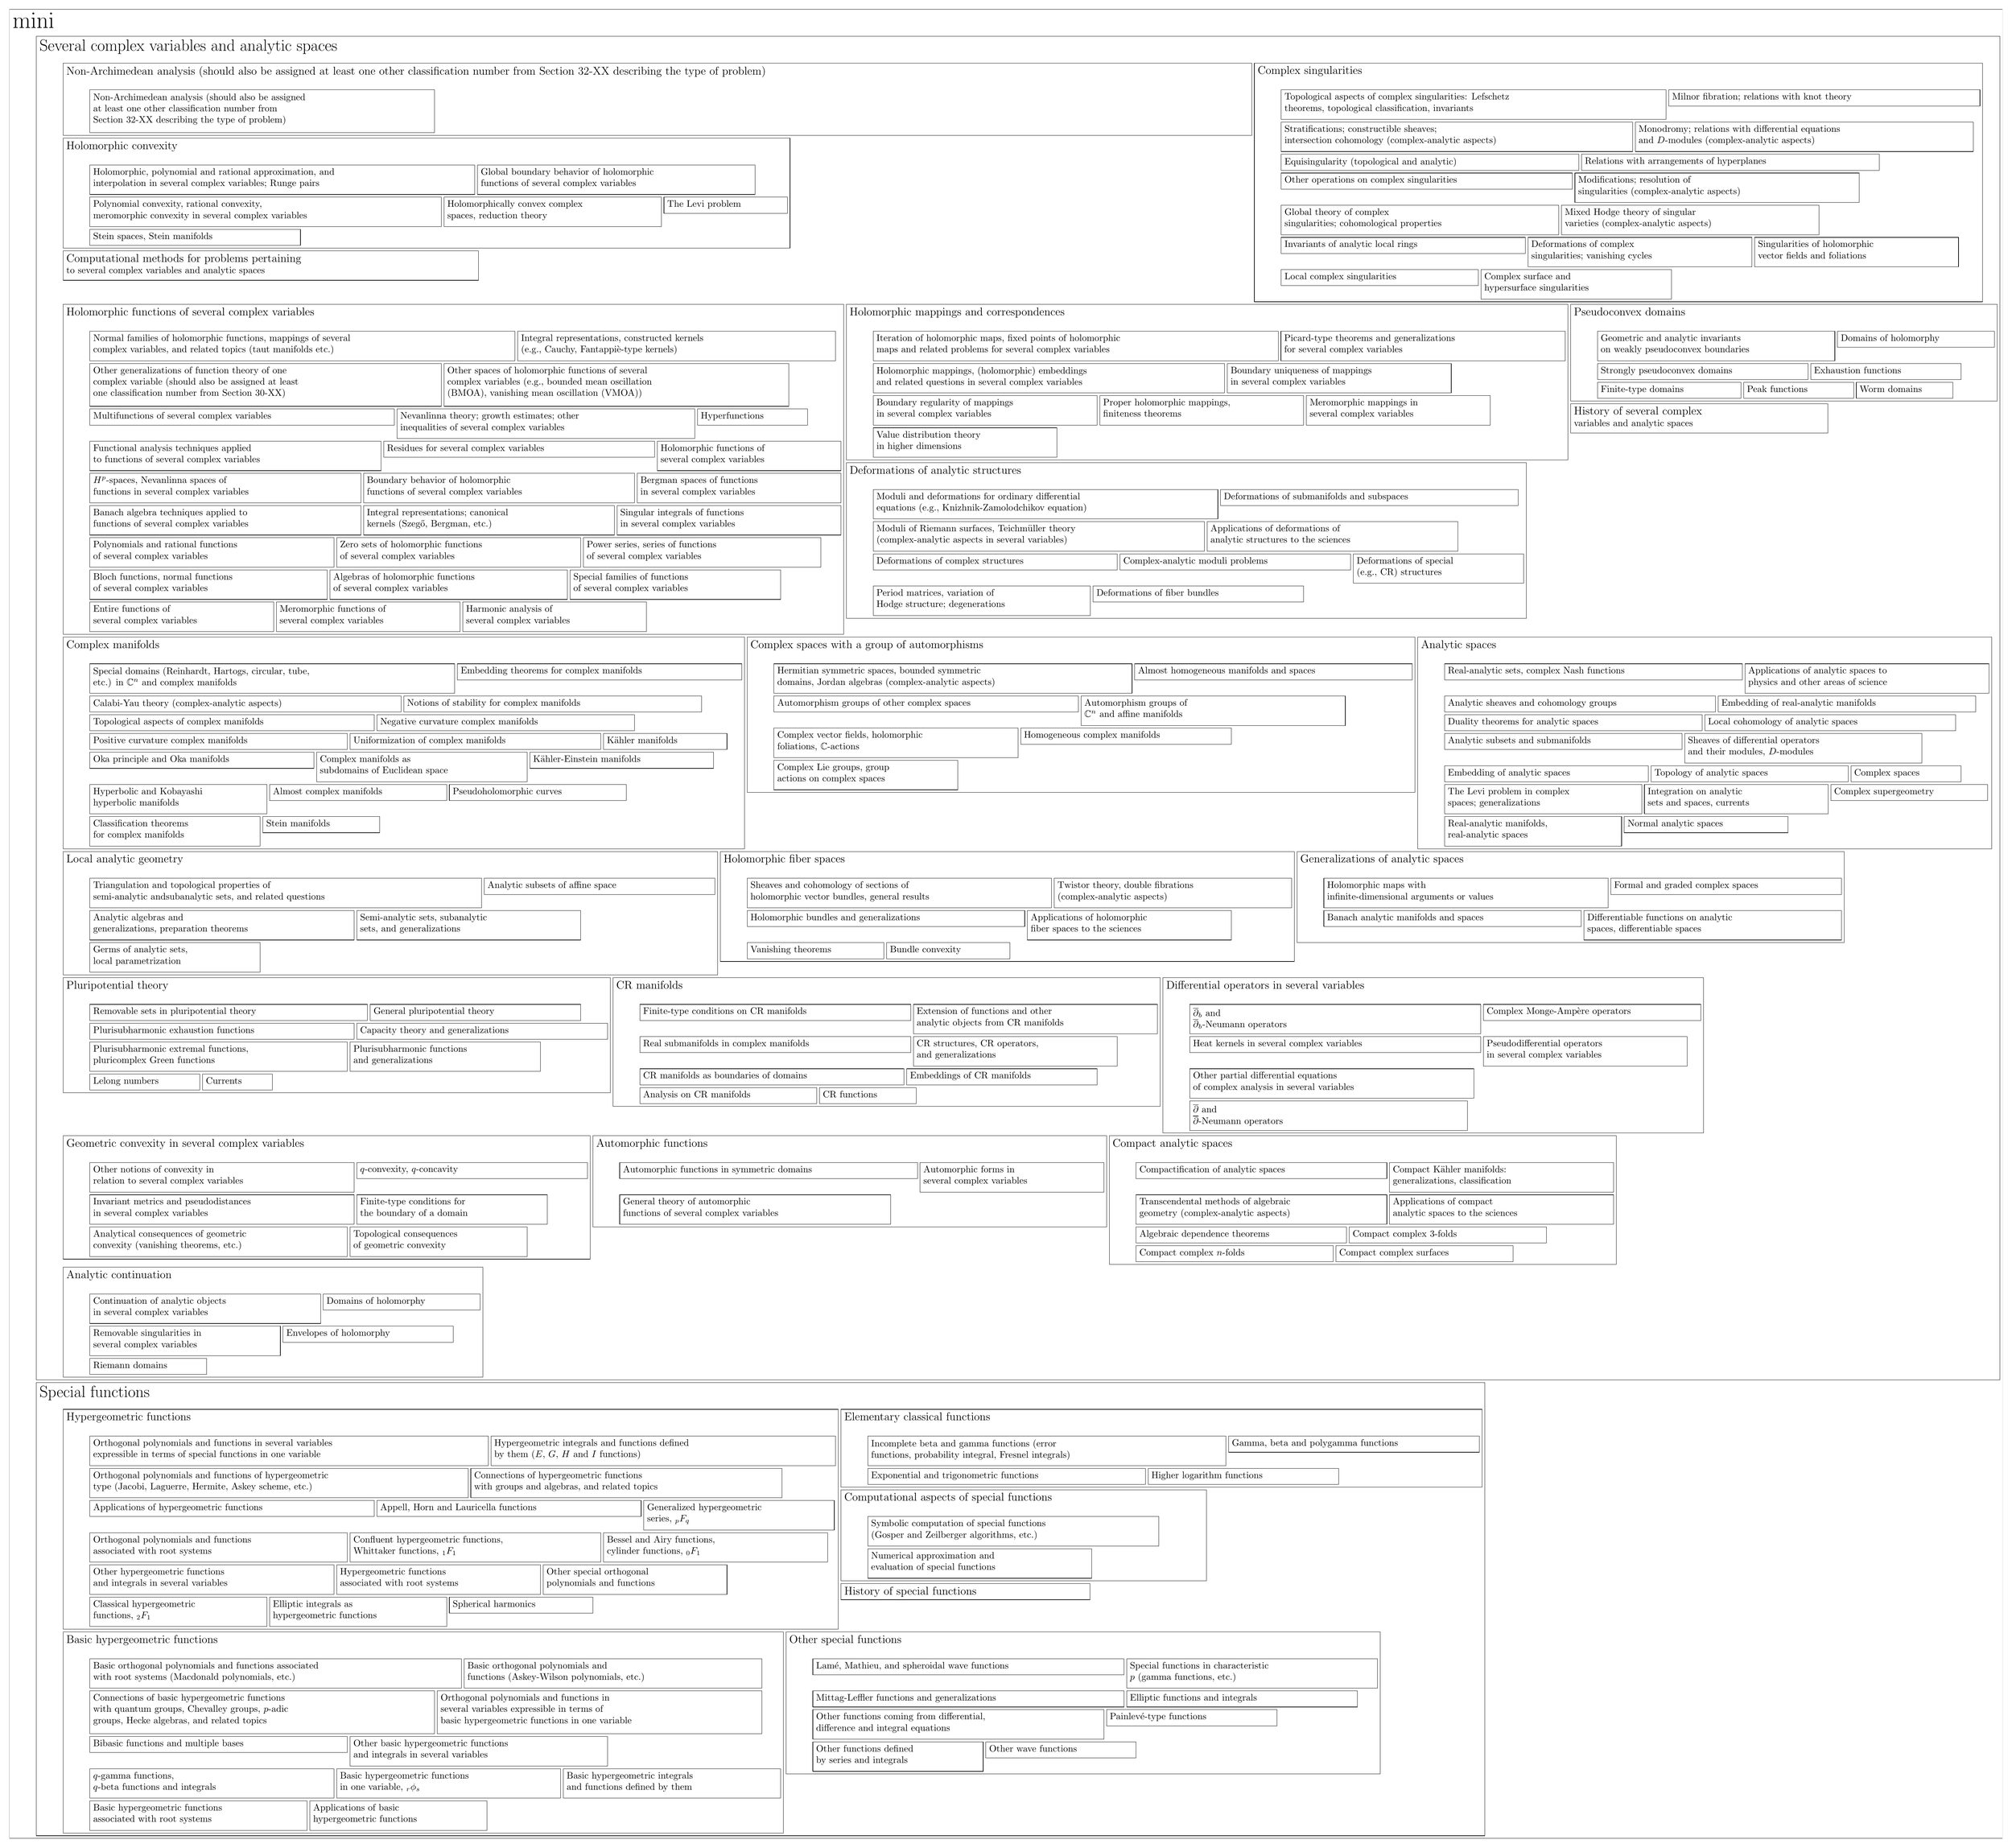
\begin{tikzpicture}[line cap=round,line join=round,>=triangle 45,x=1cm,y=1cm]
\clip(0, 0)rectangle(74.3, -68.19999999999999);

\draw(0, 0) node[anchor=north west,align=left] {\Huge mini};
\draw (0, 0) rectangle (74.3,-68.19999999999999);
\draw(1, -1) node[anchor=north west,align=left] {\LARGE Several complex variables and analytic spaces};
\draw (1, -1) rectangle (74.2,-51.099999999999994);
\draw(2, -2) node[anchor=north west,align=left] {\large Non-Archimedean analysis (should also be assigned at least one other classification number from Section 32-XX describing the type of problem)};
\draw (2, -2) rectangle (46.31,-4.7);
\draw(3, -3) node[anchor=north west,align=left] {Non-Archimedean analysis (should also be assigned\\ at least one other classification number from\\ Section 32-XX describing the type of problem)};
\draw (3, -3) rectangle (15.85,-4.6);
\draw(46.410000000000004, -2) node[anchor=north west,align=left] {\large Complex singularities};
\draw (46.410000000000004, -2) rectangle (73.56,-10.9);
\draw(47.410000000000004, -3) node[anchor=north west,align=left] {Topological aspects of complex singularities: Lefschetz\\ theorems, topological classification, invariants};
\draw (47.410000000000004, -3) rectangle (61.760000000000005,-4.1);
\draw(61.86, -3) node[anchor=north west,align=left] {Milnor fibration; relations with knot theory};
\draw (61.86, -3) rectangle (73.46,-3.6);
\draw(47.410000000000004, -4.2) node[anchor=north west,align=left] {Stratifications; constructible sheaves; \\ intersection cohomology (complex-analytic aspects)};
\draw (47.410000000000004, -4.2) rectangle (60.510000000000005,-5.300000000000001);
\draw(60.61, -4.2) node[anchor=north west,align=left] {Monodromy; relations with differential equations\\ and \(D\)-modules (complex-analytic aspects)};
\draw (60.61, -4.2) rectangle (73.21,-5.300000000000001);
\draw(47.410000000000004, -5.4) node[anchor=north west,align=left] {Equisingularity (topological and analytic)};
\draw (47.410000000000004, -5.4) rectangle (58.510000000000005,-6.0);
\draw(58.61, -5.4) node[anchor=north west,align=left] {Relations with arrangements of hyperplanes};
\draw (58.61, -5.4) rectangle (69.71,-6.0);
\draw(47.410000000000004, -6.1000000000000005) node[anchor=north west,align=left] {Other operations on complex singularities};
\draw (47.410000000000004, -6.1000000000000005) rectangle (58.260000000000005,-6.7);
\draw(58.36, -6.1000000000000005) node[anchor=north west,align=left] {Modifications; resolution of \\ singularities (complex-analytic aspects)};
\draw (58.36, -6.1000000000000005) rectangle (68.96,-7.200000000000001);
\draw(47.410000000000004, -7.300000000000001) node[anchor=north west,align=left] {Global theory of complex \\ singularities; cohomological properties};
\draw (47.410000000000004, -7.300000000000001) rectangle (57.760000000000005,-8.4);
\draw(57.86, -7.300000000000001) node[anchor=north west,align=left] {Mixed Hodge theory of singular \\ varieties (complex-analytic aspects)};
\draw (57.86, -7.300000000000001) rectangle (67.46,-8.4);
\draw(47.410000000000004, -8.5) node[anchor=north west,align=left] {Invariants of analytic local rings};
\draw (47.410000000000004, -8.5) rectangle (56.510000000000005,-9.1);
\draw(56.61, -8.5) node[anchor=north west,align=left] {Deformations of complex \\ singularities; vanishing cycles};
\draw (56.61, -8.5) rectangle (64.96,-9.6);
\draw(65.06, -8.5) node[anchor=north west,align=left] {Singularities of holomorphic\\ vector fields and foliations};
\draw (65.06, -8.5) rectangle (72.66,-9.6);
\draw(47.410000000000004, -9.700000000000001) node[anchor=north west,align=left] {Local complex singularities};
\draw (47.410000000000004, -9.700000000000001) rectangle (54.760000000000005,-10.3);
\draw(54.86, -9.700000000000001) node[anchor=north west,align=left] {Complex surface and \\ hypersurface singularities};
\draw (54.86, -9.700000000000001) rectangle (61.96,-10.8);
\draw(2, -4.800000000000001) node[anchor=north west,align=left] {\large Holomorphic convexity};
\draw (2, -4.800000000000001) rectangle (29.1,-8.9);
\draw(3, -5.800000000000001) node[anchor=north west,align=left] {Holomorphic, polynomial and rational approximation, and\\ interpolation in several complex variables; Runge pairs};
\draw (3, -5.800000000000001) rectangle (17.35,-6.9);
\draw(17.45, -5.800000000000001) node[anchor=north west,align=left] {Global boundary behavior of holomorphic\\ functions of several complex variables};
\draw (17.45, -5.800000000000001) rectangle (27.799999999999997,-6.9);
\draw(3, -7.000000000000001) node[anchor=north west,align=left] {Polynomial convexity, rational convexity, \\ meromorphic convexity in several complex variables};
\draw (3, -7.000000000000001) rectangle (16.1,-8.100000000000001);
\draw(16.2, -7.000000000000001) node[anchor=north west,align=left] {Holomorphically convex complex\\ spaces, reduction theory};
\draw (16.2, -7.000000000000001) rectangle (24.299999999999997,-8.100000000000001);
\draw(24.4, -7.000000000000001) node[anchor=north west,align=left] {The Levi problem};
\draw (24.4, -7.000000000000001) rectangle (29.0,-7.6000000000000005);
\draw(3, -8.200000000000001) node[anchor=north west,align=left] {Stein spaces, Stein manifolds};
\draw (3, -8.200000000000001) rectangle (10.85,-8.8);
\draw(2, -9.0) node[anchor=north west,align=left] {\large Computational methods for problems pertaining \\ to several complex variables and analytic spaces};
\draw (2, -9.0) rectangle (17.479999999999997,-10.1);
\draw(2, -11.0) node[anchor=north west,align=left] {\large Holomorphic functions of several complex variables};
\draw (2, -11.0) rectangle (31.1,-23.3);
\draw(3, -12.0) node[anchor=north west,align=left] {Normal families of holomorphic functions, mappings of several\\ complex variables, and related topics (taut manifolds etc.)};
\draw (3, -12.0) rectangle (18.85,-13.1);
\draw(18.950000000000003, -12.0) node[anchor=north west,align=left] {Integral representations, constructed kernels\\ (e.g., Cauchy, Fantappiè-type kernels)};
\draw (18.950000000000003, -12.0) rectangle (30.800000000000004,-13.1);
\draw(3, -13.2) node[anchor=north west,align=left] {Other generalizations of function theory of one\\ complex variable (should also be assigned at least\\ one classification number from Section 30-XX)};
\draw (3, -13.2) rectangle (16.1,-14.799999999999999);
\draw(16.2, -13.2) node[anchor=north west,align=left] {Other spaces of holomorphic functions of several\\ complex variables (e.g., bounded mean oscillation\\ (BMOA), vanishing mean oscillation (VMOA))};
\draw (16.2, -13.2) rectangle (29.049999999999997,-14.799999999999999);
\draw(3, -14.9) node[anchor=north west,align=left] {Multifunctions of several complex variables};
\draw (3, -14.9) rectangle (14.35,-15.5);
\draw(14.45, -14.9) node[anchor=north west,align=left] {Nevanlinna theory; growth estimates; other\\ inequalities of several complex variables};
\draw (14.45, -14.9) rectangle (25.549999999999997,-16.0);
\draw(25.65, -14.9) node[anchor=north west,align=left] {Hyperfunctions};
\draw (25.65, -14.9) rectangle (29.75,-15.5);
\draw(3, -16.1) node[anchor=north west,align=left] {Functional analysis techniques applied \\ to functions of several complex variables};
\draw (3, -16.1) rectangle (13.85,-17.200000000000003);
\draw(13.95, -16.1) node[anchor=north west,align=left] {Residues for several complex variables};
\draw (13.95, -16.1) rectangle (24.049999999999997,-16.700000000000003);
\draw(24.15, -16.1) node[anchor=north west,align=left] {Holomorphic functions of\\ several complex variables};
\draw (24.15, -16.1) rectangle (31.0,-17.200000000000003);
\draw(3, -17.3) node[anchor=north west,align=left] {\(H^p\)-spaces, Nevanlinna spaces of\\ functions in several complex variables};
\draw (3, -17.3) rectangle (13.1,-18.400000000000002);
\draw(13.2, -17.3) node[anchor=north west,align=left] {Boundary behavior of holomorphic \\ functions of several complex variables};
\draw (13.2, -17.3) rectangle (23.299999999999997,-18.400000000000002);
\draw(23.4, -17.3) node[anchor=north west,align=left] {Bergman spaces of functions\\ in several complex variables};
\draw (23.4, -17.3) rectangle (31.0,-18.400000000000002);
\draw(3, -18.5) node[anchor=north west,align=left] {Banach algebra techniques applied to\\ functions of several complex variables};
\draw (3, -18.5) rectangle (13.1,-19.6);
\draw(13.2, -18.5) node[anchor=north west,align=left] {Integral representations; canonical\\ kernels (Szegő, Bergman, etc.)};
\draw (13.2, -18.5) rectangle (22.549999999999997,-19.6);
\draw(22.65, -18.5) node[anchor=north west,align=left] {Singular integrals of functions\\ in several complex variables};
\draw (22.65, -18.5) rectangle (31.0,-19.6);
\draw(3, -19.700000000000003) node[anchor=north west,align=left] {Polynomials and rational functions\\ of several complex variables};
\draw (3, -19.700000000000003) rectangle (12.1,-20.800000000000004);
\draw(12.2, -19.700000000000003) node[anchor=north west,align=left] {Zero sets of holomorphic functions\\ of several complex variables};
\draw (12.2, -19.700000000000003) rectangle (21.299999999999997,-20.800000000000004);
\draw(21.4, -19.700000000000003) node[anchor=north west,align=left] {Power series, series of functions\\ of several complex variables};
\draw (21.4, -19.700000000000003) rectangle (30.25,-20.800000000000004);
\draw(3, -20.900000000000002) node[anchor=north west,align=left] {Bloch functions, normal functions\\ of several complex variables};
\draw (3, -20.900000000000002) rectangle (11.85,-22.000000000000004);
\draw(11.95, -20.900000000000002) node[anchor=north west,align=left] {Algebras of holomorphic functions\\ of several complex variables};
\draw (11.95, -20.900000000000002) rectangle (20.799999999999997,-22.000000000000004);
\draw(20.9, -20.900000000000002) node[anchor=north west,align=left] {Special families of functions\\ of several complex variables};
\draw (20.9, -20.900000000000002) rectangle (28.75,-22.000000000000004);
\draw(3, -22.1) node[anchor=north west,align=left] {Entire functions of \\ several complex variables};
\draw (3, -22.1) rectangle (9.85,-23.200000000000003);
\draw(9.95, -22.1) node[anchor=north west,align=left] {Meromorphic functions of\\ several complex variables};
\draw (9.95, -22.1) rectangle (16.799999999999997,-23.200000000000003);
\draw(16.9, -22.1) node[anchor=north west,align=left] {Harmonic analysis of \\ several complex variables};
\draw (16.9, -22.1) rectangle (23.75,-23.200000000000003);
\draw(31.200000000000003, -11.0) node[anchor=north west,align=left] {\large Holomorphic mappings and correspondences};
\draw (31.200000000000003, -11.0) rectangle (58.10000000000001,-16.8);
\draw(32.2, -12.0) node[anchor=north west,align=left] {Iteration of holomorphic maps, fixed points of holomorphic\\ maps and related problems for several complex variables};
\draw (32.2, -12.0) rectangle (47.300000000000004,-13.1);
\draw(47.400000000000006, -12.0) node[anchor=north west,align=left] {Picard-type theorems and generalizations\\ for several complex variables};
\draw (47.400000000000006, -12.0) rectangle (58.00000000000001,-13.1);
\draw(32.2, -13.2) node[anchor=north west,align=left] {Holomorphic mappings, (holomorphic) embeddings \\ and related questions in several complex variables};
\draw (32.2, -13.2) rectangle (45.300000000000004,-14.299999999999999);
\draw(45.400000000000006, -13.2) node[anchor=north west,align=left] {Boundary uniqueness of mappings\\ in several complex variables};
\draw (45.400000000000006, -13.2) rectangle (53.75000000000001,-14.299999999999999);
\draw(32.2, -14.4) node[anchor=north west,align=left] {Boundary regularity of mappings\\ in several complex variables};
\draw (32.2, -14.4) rectangle (40.550000000000004,-15.5);
\draw(40.650000000000006, -14.4) node[anchor=north west,align=left] {Proper holomorphic mappings,\\ finiteness theorems};
\draw (40.650000000000006, -14.4) rectangle (48.25000000000001,-15.5);
\draw(48.35, -14.4) node[anchor=north west,align=left] {Meromorphic mappings in\\ several complex variables};
\draw (48.35, -14.4) rectangle (55.2,-15.5);
\draw(32.2, -15.600000000000001) node[anchor=north west,align=left] {Value distribution theory\\ in higher dimensions};
\draw (32.2, -15.600000000000001) rectangle (39.050000000000004,-16.700000000000003);
\draw(31.200000000000003, -16.9) node[anchor=north west,align=left] {\large Deformations of analytic structures};
\draw (31.200000000000003, -16.9) rectangle (56.550000000000004,-22.7);
\draw(32.2, -17.9) node[anchor=north west,align=left] {Moduli and deformations for ordinary differential\\ equations (e.g., Knizhnik-Zamolodchikov equation)};
\draw (32.2, -17.9) rectangle (45.050000000000004,-19.0);
\draw(45.150000000000006, -17.9) node[anchor=north west,align=left] {Deformations of submanifolds and subspaces};
\draw (45.150000000000006, -17.9) rectangle (56.25000000000001,-18.5);
\draw(32.2, -19.099999999999998) node[anchor=north west,align=left] {Moduli of Riemann surfaces, Teichmüller theory\\ (complex-analytic aspects in several variables)};
\draw (32.2, -19.099999999999998) rectangle (44.550000000000004,-20.2);
\draw(44.650000000000006, -19.099999999999998) node[anchor=north west,align=left] {Applications of deformations of \\ analytic structures to the sciences};
\draw (44.650000000000006, -19.099999999999998) rectangle (54.00000000000001,-20.2);
\draw(32.2, -20.299999999999997) node[anchor=north west,align=left] {Deformations of complex structures};
\draw (32.2, -20.299999999999997) rectangle (41.300000000000004,-20.9);
\draw(41.400000000000006, -20.299999999999997) node[anchor=north west,align=left] {Complex-analytic moduli problems};
\draw (41.400000000000006, -20.299999999999997) rectangle (50.00000000000001,-20.9);
\draw(50.1, -20.299999999999997) node[anchor=north west,align=left] {Deformations of special\\ (e.g., CR) structures};
\draw (50.1, -20.299999999999997) rectangle (56.45,-21.4);
\draw(32.2, -21.5) node[anchor=north west,align=left] {Period matrices, variation of\\ Hodge structure; degenerations};
\draw (32.2, -21.5) rectangle (40.300000000000004,-22.6);
\draw(40.400000000000006, -21.5) node[anchor=north west,align=left] {Deformations of fiber bundles};
\draw (40.400000000000006, -21.5) rectangle (48.25000000000001,-22.1);
\draw(58.20000000000001, -11.0) node[anchor=north west,align=left] {\large Pseudoconvex domains};
\draw (58.20000000000001, -11.0) rectangle (74.10000000000001,-14.600000000000001);
\draw(59.20000000000001, -12.0) node[anchor=north west,align=left] {Geometric and analytic invariants\\ on weakly pseudoconvex boundaries};
\draw (59.20000000000001, -12.0) rectangle (68.05000000000001,-13.1);
\draw(68.15, -12.0) node[anchor=north west,align=left] {Domains of holomorphy};
\draw (68.15, -12.0) rectangle (74.0,-12.6);
\draw(59.20000000000001, -13.2) node[anchor=north west,align=left] {Strongly pseudoconvex domains};
\draw (59.20000000000001, -13.2) rectangle (67.05000000000001,-13.799999999999999);
\draw(67.15, -13.2) node[anchor=north west,align=left] {Exhaustion functions};
\draw (67.15, -13.2) rectangle (72.75,-13.799999999999999);
\draw(59.20000000000001, -13.9) node[anchor=north west,align=left] {Finite-type domains};
\draw (59.20000000000001, -13.9) rectangle (64.55000000000001,-14.5);
\draw(64.65, -13.9) node[anchor=north west,align=left] {Peak functions};
\draw (64.65, -13.9) rectangle (68.75,-14.5);
\draw(68.85000000000001, -13.9) node[anchor=north west,align=left] {Worm domains};
\draw (68.85000000000001, -13.9) rectangle (72.45,-14.5);
\draw(58.20000000000001, -14.700000000000001) node[anchor=north west,align=left] {\large History of several complex \\ variables and analytic spaces};
\draw (58.20000000000001, -14.700000000000001) rectangle (67.79,-15.8);
\draw(2, -23.4) node[anchor=north west,align=left] {\large Complex manifolds};
\draw (2, -23.4) rectangle (27.4,-31.299999999999997);
\draw(3, -24.4) node[anchor=north west,align=left] {Special domains (Reinhardt, Hartogs, circular, tube,\\ etc.) in \(\mathbb{C}^n\) and complex manifolds};
\draw (3, -24.4) rectangle (16.6,-25.5);
\draw(16.7, -24.4) node[anchor=north west,align=left] {Embedding theorems for complex manifolds};
\draw (16.7, -24.4) rectangle (27.299999999999997,-25.0);
\draw(3, -25.599999999999998) node[anchor=north west,align=left] {Calabi-Yau theory (complex-analytic aspects)};
\draw (3, -25.599999999999998) rectangle (14.6,-26.2);
\draw(14.7, -25.599999999999998) node[anchor=north west,align=left] {Notions of stability for complex manifolds};
\draw (14.7, -25.599999999999998) rectangle (25.799999999999997,-26.2);
\draw(3, -26.299999999999997) node[anchor=north west,align=left] {Topological aspects of complex manifolds};
\draw (3, -26.299999999999997) rectangle (13.6,-26.9);
\draw(13.7, -26.299999999999997) node[anchor=north west,align=left] {Negative curvature complex manifolds};
\draw (13.7, -26.299999999999997) rectangle (23.299999999999997,-26.9);
\draw(3, -27.0) node[anchor=north west,align=left] {Positive curvature complex manifolds};
\draw (3, -27.0) rectangle (12.6,-27.6);
\draw(12.7, -27.0) node[anchor=north west,align=left] {Uniformization of complex manifolds};
\draw (12.7, -27.0) rectangle (22.049999999999997,-27.6);
\draw(22.15, -27.0) node[anchor=north west,align=left] {Kähler manifolds};
\draw (22.15, -27.0) rectangle (26.75,-27.6);
\draw(3, -27.7) node[anchor=north west,align=left] {Oka principle and Oka manifolds};
\draw (3, -27.7) rectangle (11.35,-28.3);
\draw(11.45, -27.7) node[anchor=north west,align=left] {Complex manifolds as \\ subdomains of Euclidean space};
\draw (11.45, -27.7) rectangle (19.299999999999997,-28.8);
\draw(19.4, -27.7) node[anchor=north west,align=left] {Kähler-Einstein manifolds};
\draw (19.4, -27.7) rectangle (26.25,-28.3);
\draw(3, -28.9) node[anchor=north west,align=left] {Hyperbolic and Kobayashi\\ hyperbolic manifolds};
\draw (3, -28.9) rectangle (9.6,-30.0);
\draw(9.7, -28.9) node[anchor=north west,align=left] {Almost complex manifolds};
\draw (9.7, -28.9) rectangle (16.299999999999997,-29.5);
\draw(16.4, -28.9) node[anchor=north west,align=left] {Pseudoholomorphic curves};
\draw (16.4, -28.9) rectangle (23.0,-29.5);
\draw(3, -30.1) node[anchor=north west,align=left] {Classification theorems\\ for complex manifolds};
\draw (3, -30.1) rectangle (9.35,-31.200000000000003);
\draw(9.45, -30.1) node[anchor=north west,align=left] {Stein manifolds};
\draw (9.45, -30.1) rectangle (13.799999999999999,-30.700000000000003);
\draw(27.5, -23.4) node[anchor=north west,align=left] {\large Complex spaces with a group of automorphisms};
\draw (27.5, -23.4) rectangle (52.4,-29.2);
\draw(28.5, -24.4) node[anchor=north west,align=left] {Hermitian symmetric spaces, bounded symmetric \\ domains, Jordan algebras (complex-analytic aspects)};
\draw (28.5, -24.4) rectangle (41.85,-25.5);
\draw(41.95, -24.4) node[anchor=north west,align=left] {Almost homogeneous manifolds and spaces};
\draw (41.95, -24.4) rectangle (52.300000000000004,-25.0);
\draw(28.5, -25.599999999999998) node[anchor=north west,align=left] {Automorphism groups of other complex spaces};
\draw (28.5, -25.599999999999998) rectangle (39.85,-26.2);
\draw(39.95, -25.599999999999998) node[anchor=north west,align=left] {Automorphism groups of \\ \(\mathbb{C}^n\) and affine manifolds};
\draw (39.95, -25.599999999999998) rectangle (49.800000000000004,-26.7);
\draw(28.5, -26.799999999999997) node[anchor=north west,align=left] {Complex vector fields, holomorphic\\ foliations, \(\mathbb{C}\)-actions};
\draw (28.5, -26.799999999999997) rectangle (37.6,-27.9);
\draw(37.7, -26.799999999999997) node[anchor=north west,align=left] {Homogeneous complex manifolds};
\draw (37.7, -26.799999999999997) rectangle (45.550000000000004,-27.4);
\draw(28.5, -28.0) node[anchor=north west,align=left] {Complex Lie groups, group\\ actions on complex spaces};
\draw (28.5, -28.0) rectangle (35.35,-29.1);
\draw(52.5, -23.4) node[anchor=north west,align=left] {\large Analytic spaces};
\draw (52.5, -23.4) rectangle (73.9,-31.299999999999997);
\draw(53.5, -24.4) node[anchor=north west,align=left] {Real-analytic sets, complex Nash functions};
\draw (53.5, -24.4) rectangle (64.6,-25.0);
\draw(64.7, -24.4) node[anchor=north west,align=left] {Applications of analytic spaces to\\ physics and other areas of science};
\draw (64.7, -24.4) rectangle (73.8,-25.5);
\draw(53.5, -25.599999999999998) node[anchor=north west,align=left] {Analytic sheaves and cohomology groups};
\draw (53.5, -25.599999999999998) rectangle (63.6,-26.2);
\draw(63.7, -25.599999999999998) node[anchor=north west,align=left] {Embedding of real-analytic manifolds};
\draw (63.7, -25.599999999999998) rectangle (73.3,-26.2);
\draw(53.5, -26.299999999999997) node[anchor=north west,align=left] {Duality theorems for analytic spaces};
\draw (53.5, -26.299999999999997) rectangle (63.1,-26.9);
\draw(63.2, -26.299999999999997) node[anchor=north west,align=left] {Local cohomology of analytic spaces};
\draw (63.2, -26.299999999999997) rectangle (72.55,-26.9);
\draw(53.5, -27.0) node[anchor=north west,align=left] {Analytic subsets and submanifolds};
\draw (53.5, -27.0) rectangle (62.35,-27.6);
\draw(62.45, -27.0) node[anchor=north west,align=left] {Sheaves of differential operators\\ and their modules, \(D\)-modules};
\draw (62.45, -27.0) rectangle (71.3,-28.1);
\draw(53.5, -28.2) node[anchor=north west,align=left] {Embedding of analytic spaces};
\draw (53.5, -28.2) rectangle (61.1,-28.8);
\draw(61.2, -28.2) node[anchor=north west,align=left] {Topology of analytic spaces};
\draw (61.2, -28.2) rectangle (68.55,-28.8);
\draw(68.65, -28.2) node[anchor=north west,align=left] {Complex spaces};
\draw (68.65, -28.2) rectangle (72.75,-28.8);
\draw(53.5, -28.9) node[anchor=north west,align=left] {The Levi problem in complex\\ spaces; generalizations};
\draw (53.5, -28.9) rectangle (60.85,-30.0);
\draw(60.95, -28.9) node[anchor=north west,align=left] {Integration on analytic\\ sets and spaces, currents};
\draw (60.95, -28.9) rectangle (67.8,-30.0);
\draw(67.9, -28.9) node[anchor=north west,align=left] {Complex supergeometry};
\draw (67.9, -28.9) rectangle (73.75,-29.5);
\draw(53.5, -30.1) node[anchor=north west,align=left] {Real-analytic manifolds,\\ real-analytic spaces};
\draw (53.5, -30.1) rectangle (60.1,-31.200000000000003);
\draw(60.2, -30.1) node[anchor=north west,align=left] {Normal analytic spaces};
\draw (60.2, -30.1) rectangle (66.3,-30.700000000000003);
\draw(2, -31.4) node[anchor=north west,align=left] {\large Local analytic geometry};
\draw (2, -31.4) rectangle (26.4,-36.0);
\draw(3, -32.4) node[anchor=north west,align=left] {Triangulation and topological properties of \\ semi-analytic andsubanalytic sets, and related questions};
\draw (3, -32.4) rectangle (17.6,-33.5);
\draw(17.7, -32.4) node[anchor=north west,align=left] {Analytic subsets of affine space};
\draw (17.7, -32.4) rectangle (26.299999999999997,-33.0);
\draw(3, -33.6) node[anchor=north west,align=left] {Analytic algebras and \\ generalizations, preparation theorems};
\draw (3, -33.6) rectangle (12.85,-34.7);
\draw(12.95, -33.6) node[anchor=north west,align=left] {Semi-analytic sets, subanalytic\\ sets, and generalizations};
\draw (12.95, -33.6) rectangle (21.299999999999997,-34.7);
\draw(3, -34.8) node[anchor=north west,align=left] {Germs of analytic sets,\\ local parametrization};
\draw (3, -34.8) rectangle (9.35,-35.9);
\draw(26.5, -31.4) node[anchor=north west,align=left] {\large Holomorphic fiber spaces};
\draw (26.5, -31.4) rectangle (47.9,-35.5);
\draw(27.5, -32.4) node[anchor=north west,align=left] {Sheaves and cohomology of sections of \\ holomorphic vector bundles, general results};
\draw (27.5, -32.4) rectangle (38.85,-33.5);
\draw(38.95, -32.4) node[anchor=north west,align=left] {Twistor theory, double fibrations\\ (complex-analytic aspects)};
\draw (38.95, -32.4) rectangle (47.800000000000004,-33.5);
\draw(27.5, -33.6) node[anchor=north west,align=left] {Holomorphic bundles and generalizations};
\draw (27.5, -33.6) rectangle (37.85,-34.2);
\draw(37.95, -33.6) node[anchor=north west,align=left] {Applications of holomorphic\\ fiber spaces to the sciences};
\draw (37.95, -33.6) rectangle (45.550000000000004,-34.7);
\draw(27.5, -34.8) node[anchor=north west,align=left] {Vanishing theorems};
\draw (27.5, -34.8) rectangle (32.6,-35.4);
\draw(32.7, -34.8) node[anchor=north west,align=left] {Bundle convexity};
\draw (32.7, -34.8) rectangle (37.300000000000004,-35.4);
\draw(48.0, -31.4) node[anchor=north west,align=left] {\large Generalizations of analytic spaces};
\draw (48.0, -31.4) rectangle (68.4,-34.8);
\draw(49.0, -32.4) node[anchor=north west,align=left] {Holomorphic maps with \\ infinite-dimensional arguments or values};
\draw (49.0, -32.4) rectangle (59.6,-33.5);
\draw(59.7, -32.4) node[anchor=north west,align=left] {Formal and graded complex spaces};
\draw (59.7, -32.4) rectangle (68.3,-33.0);
\draw(49.0, -33.6) node[anchor=north west,align=left] {Banach analytic manifolds and spaces};
\draw (49.0, -33.6) rectangle (58.6,-34.2);
\draw(58.7, -33.6) node[anchor=north west,align=left] {Differentiable functions on analytic\\ spaces, differentiable spaces};
\draw (58.7, -33.6) rectangle (68.3,-34.7);
\draw(2, -36.099999999999994) node[anchor=north west,align=left] {\large Pluripotential theory};
\draw (2, -36.099999999999994) rectangle (22.4,-40.39999999999999);
\draw(3, -37.099999999999994) node[anchor=north west,align=left] {Removable sets in pluripotential theory};
\draw (3, -37.099999999999994) rectangle (13.35,-37.699999999999996);
\draw(13.45, -37.099999999999994) node[anchor=north west,align=left] {General pluripotential theory};
\draw (13.45, -37.099999999999994) rectangle (21.299999999999997,-37.699999999999996);
\draw(3, -37.8) node[anchor=north west,align=left] {Plurisubharmonic exhaustion functions};
\draw (3, -37.8) rectangle (12.85,-38.4);
\draw(12.95, -37.8) node[anchor=north west,align=left] {Capacity theory and generalizations};
\draw (12.95, -37.8) rectangle (22.299999999999997,-38.4);
\draw(3, -38.49999999999999) node[anchor=north west,align=left] {Plurisubharmonic extremal functions,\\ pluricomplex Green functions};
\draw (3, -38.49999999999999) rectangle (12.6,-39.599999999999994);
\draw(12.7, -38.49999999999999) node[anchor=north west,align=left] {Plurisubharmonic functions\\ and generalizations};
\draw (12.7, -38.49999999999999) rectangle (19.799999999999997,-39.599999999999994);
\draw(3, -39.699999999999996) node[anchor=north west,align=left] {Lelong numbers};
\draw (3, -39.699999999999996) rectangle (7.1,-40.3);
\draw(7.199999999999999, -39.699999999999996) node[anchor=north west,align=left] {Currents};
\draw (7.199999999999999, -39.699999999999996) rectangle (9.799999999999999,-40.3);
\draw(22.5, -36.099999999999994) node[anchor=north west,align=left] {\large CR manifolds};
\draw (22.5, -36.099999999999994) rectangle (42.9,-40.89999999999999);
\draw(23.5, -37.099999999999994) node[anchor=north west,align=left] {Finite-type conditions on CR manifolds};
\draw (23.5, -37.099999999999994) rectangle (33.6,-37.699999999999996);
\draw(33.7, -37.099999999999994) node[anchor=north west,align=left] {Extension of functions and other\\ analytic objects from CR manifolds};
\draw (33.7, -37.099999999999994) rectangle (42.800000000000004,-38.199999999999996);
\draw(23.5, -38.3) node[anchor=north west,align=left] {Real submanifolds in complex manifolds};
\draw (23.5, -38.3) rectangle (33.6,-38.9);
\draw(33.7, -38.3) node[anchor=north west,align=left] {CR structures, CR operators,\\ and generalizations};
\draw (33.7, -38.3) rectangle (41.300000000000004,-39.4);
\draw(23.5, -39.49999999999999) node[anchor=north west,align=left] {CR manifolds as boundaries of domains};
\draw (23.5, -39.49999999999999) rectangle (33.35,-40.099999999999994);
\draw(33.45, -39.49999999999999) node[anchor=north west,align=left] {Embeddings of CR manifolds};
\draw (33.45, -39.49999999999999) rectangle (40.550000000000004,-40.099999999999994);
\draw(23.5, -40.199999999999996) node[anchor=north west,align=left] {Analysis on CR manifolds};
\draw (23.5, -40.199999999999996) rectangle (30.1,-40.8);
\draw(30.2, -40.199999999999996) node[anchor=north west,align=left] {CR functions};
\draw (30.2, -40.199999999999996) rectangle (33.8,-40.8);
\draw(43.0, -36.099999999999994) node[anchor=north west,align=left] {\large Differential operators in several variables};
\draw (43.0, -36.099999999999994) rectangle (63.15,-41.89999999999999);
\draw(44.0, -37.099999999999994) node[anchor=north west,align=left] {\(\overline\partial_b\) and \\ \(\overline\partial_b\)-Neumann operators};
\draw (44.0, -37.099999999999994) rectangle (54.85,-38.199999999999996);
\draw(54.95, -37.099999999999994) node[anchor=north west,align=left] {Complex Monge-Ampère operators};
\draw (54.95, -37.099999999999994) rectangle (63.050000000000004,-37.699999999999996);
\draw(44.0, -38.3) node[anchor=north west,align=left] {Heat kernels in several complex variables};
\draw (44.0, -38.3) rectangle (54.85,-38.9);
\draw(54.95, -38.3) node[anchor=north west,align=left] {Pseudodifferential operators\\ in several complex variables};
\draw (54.95, -38.3) rectangle (62.550000000000004,-39.4);
\draw(44.0, -39.49999999999999) node[anchor=north west,align=left] {Other partial differential equations \\ of complex analysis in several variables};
\draw (44.0, -39.49999999999999) rectangle (54.6,-40.599999999999994);
\draw(44.0, -40.699999999999996) node[anchor=north west,align=left] {\(\overline\partial\) and \\ \(\overline\partial\)-Neumann operators};
\draw (44.0, -40.699999999999996) rectangle (54.35,-41.8);
\draw(2, -41.99999999999999) node[anchor=north west,align=left] {\large Geometric convexity in several complex variables};
\draw (2, -41.99999999999999) rectangle (21.65,-46.599999999999994);
\draw(3, -42.99999999999999) node[anchor=north west,align=left] {Other notions of convexity in \\ relation to several complex variables};
\draw (3, -42.99999999999999) rectangle (12.85,-44.099999999999994);
\draw(12.95, -42.99999999999999) node[anchor=north west,align=left] {\(q\)-convexity, \(q\)-concavity};
\draw (12.95, -42.99999999999999) rectangle (21.549999999999997,-43.599999999999994);
\draw(3, -44.199999999999996) node[anchor=north west,align=left] {Invariant metrics and pseudodistances\\ in several complex variables};
\draw (3, -44.199999999999996) rectangle (12.85,-45.3);
\draw(12.95, -44.199999999999996) node[anchor=north west,align=left] {Finite-type conditions for\\ the boundary of a domain};
\draw (12.95, -44.199999999999996) rectangle (20.049999999999997,-45.3);
\draw(3, -45.39999999999999) node[anchor=north west,align=left] {Analytical consequences of geometric\\ convexity (vanishing theorems, etc.)};
\draw (3, -45.39999999999999) rectangle (12.6,-46.49999999999999);
\draw(12.7, -45.39999999999999) node[anchor=north west,align=left] {Topological consequences\\ of geometric convexity};
\draw (12.7, -45.39999999999999) rectangle (19.299999999999997,-46.49999999999999);
\draw(21.75, -41.99999999999999) node[anchor=north west,align=left] {\large Automorphic functions};
\draw (21.75, -41.99999999999999) rectangle (40.9,-45.39999999999999);
\draw(22.75, -42.99999999999999) node[anchor=north west,align=left] {Automorphic functions in symmetric domains};
\draw (22.75, -42.99999999999999) rectangle (33.85,-43.599999999999994);
\draw(33.95, -42.99999999999999) node[anchor=north west,align=left] {Automorphic forms in \\ several complex variables};
\draw (33.95, -42.99999999999999) rectangle (40.800000000000004,-44.099999999999994);
\draw(22.75, -44.199999999999996) node[anchor=north west,align=left] {General theory of automorphic \\ functions of several complex variables};
\draw (22.75, -44.199999999999996) rectangle (32.85,-45.3);
\draw(41.0, -41.99999999999999) node[anchor=north west,align=left] {\large Compact analytic spaces};
\draw (41.0, -41.99999999999999) rectangle (59.9,-46.79999999999999);
\draw(42.0, -42.99999999999999) node[anchor=north west,align=left] {Compactification of analytic spaces};
\draw (42.0, -42.99999999999999) rectangle (51.35,-43.599999999999994);
\draw(51.45, -42.99999999999999) node[anchor=north west,align=left] {Compact Kähler manifolds: \\ generalizations, classification};
\draw (51.45, -42.99999999999999) rectangle (59.800000000000004,-44.099999999999994);
\draw(42.0, -44.199999999999996) node[anchor=north west,align=left] {Transcendental methods of algebraic\\ geometry (complex-analytic aspects)};
\draw (42.0, -44.199999999999996) rectangle (51.35,-45.3);
\draw(51.45, -44.199999999999996) node[anchor=north west,align=left] {Applications of compact \\ analytic spaces to the sciences};
\draw (51.45, -44.199999999999996) rectangle (59.800000000000004,-45.3);
\draw(42.0, -45.39999999999999) node[anchor=north west,align=left] {Algebraic dependence theorems};
\draw (42.0, -45.39999999999999) rectangle (49.85,-45.99999999999999);
\draw(49.95, -45.39999999999999) node[anchor=north west,align=left] {Compact complex \(3\)-folds};
\draw (49.95, -45.39999999999999) rectangle (57.300000000000004,-45.99999999999999);
\draw(42.0, -46.099999999999994) node[anchor=north west,align=left] {Compact complex \(n\)-folds};
\draw (42.0, -46.099999999999994) rectangle (49.35,-46.699999999999996);
\draw(49.45, -46.099999999999994) node[anchor=north west,align=left] {Compact complex surfaces};
\draw (49.45, -46.099999999999994) rectangle (56.050000000000004,-46.699999999999996);
\draw(2, -46.89999999999999) node[anchor=north west,align=left] {\large Analytic continuation};
\draw (2, -46.89999999999999) rectangle (17.65,-50.99999999999999);
\draw(3, -47.89999999999999) node[anchor=north west,align=left] {Continuation of analytic objects\\ in several complex variables};
\draw (3, -47.89999999999999) rectangle (11.6,-48.99999999999999);
\draw(11.7, -47.89999999999999) node[anchor=north west,align=left] {Domains of holomorphy};
\draw (11.7, -47.89999999999999) rectangle (17.549999999999997,-48.49999999999999);
\draw(3, -49.099999999999994) node[anchor=north west,align=left] {Removable singularities in\\ several complex variables};
\draw (3, -49.099999999999994) rectangle (10.1,-50.199999999999996);
\draw(10.2, -49.099999999999994) node[anchor=north west,align=left] {Envelopes of holomorphy};
\draw (10.2, -49.099999999999994) rectangle (16.549999999999997,-49.699999999999996);
\draw(3, -50.29999999999999) node[anchor=north west,align=left] {Riemann domains};
\draw (3, -50.29999999999999) rectangle (7.35,-50.89999999999999);
\draw(1, -51.199999999999996) node[anchor=north west,align=left] {\LARGE Special functions};
\draw (1, -51.199999999999996) rectangle (55.0,-68.1);
\draw(2, -52.199999999999996) node[anchor=north west,align=left] {\large Hypergeometric functions};
\draw (2, -52.199999999999996) rectangle (30.9,-60.4);
\draw(3, -53.199999999999996) node[anchor=north west,align=left] {Orthogonal polynomials and functions in several variables\\ expressible in terms of special functions in one variable};
\draw (3, -53.199999999999996) rectangle (17.85,-54.3);
\draw(17.95, -53.199999999999996) node[anchor=north west,align=left] {Hypergeometric integrals and functions defined \\ by them (\(E\), \(G\), \(H\) and \(I\) functions)};
\draw (17.95, -53.199999999999996) rectangle (30.799999999999997,-54.3);
\draw(3, -54.4) node[anchor=north west,align=left] {Orthogonal polynomials and functions of hypergeometric\\ type (Jacobi, Laguerre, Hermite, Askey scheme, etc.)};
\draw (3, -54.4) rectangle (17.1,-55.5);
\draw(17.2, -54.4) node[anchor=north west,align=left] {Connections of hypergeometric functions \\ with groups and algebras, and related topics};
\draw (17.2, -54.4) rectangle (28.799999999999997,-55.5);
\draw(3, -55.599999999999994) node[anchor=north west,align=left] {Applications of hypergeometric functions};
\draw (3, -55.599999999999994) rectangle (13.6,-56.199999999999996);
\draw(13.7, -55.599999999999994) node[anchor=north west,align=left] {Appell, Horn and Lauricella functions};
\draw (13.7, -55.599999999999994) rectangle (23.549999999999997,-56.199999999999996);
\draw(23.65, -55.599999999999994) node[anchor=north west,align=left] {Generalized hypergeometric\\ series, \({}_pF_q\)};
\draw (23.65, -55.599999999999994) rectangle (30.75,-56.699999999999996);
\draw(3, -56.8) node[anchor=north west,align=left] {Orthogonal polynomials and functions\\ associated with root systems};
\draw (3, -56.8) rectangle (12.6,-57.9);
\draw(12.7, -56.8) node[anchor=north west,align=left] {Confluent hypergeometric functions,\\ Whittaker functions, \({}_1F_1\)};
\draw (12.7, -56.8) rectangle (22.049999999999997,-57.9);
\draw(22.15, -56.8) node[anchor=north west,align=left] {Bessel and Airy functions, \\ cylinder functions, \({}_0F_1\)};
\draw (22.15, -56.8) rectangle (30.5,-57.9);
\draw(3, -58.0) node[anchor=north west,align=left] {Other hypergeometric functions \\ and integrals in several variables};
\draw (3, -58.0) rectangle (12.1,-59.1);
\draw(12.2, -58.0) node[anchor=north west,align=left] {Hypergeometric functions \\ associated with root systems};
\draw (12.2, -58.0) rectangle (19.799999999999997,-59.1);
\draw(19.9, -58.0) node[anchor=north west,align=left] {Other special orthogonal\\ polynomials and functions};
\draw (19.9, -58.0) rectangle (26.75,-59.1);
\draw(3, -59.199999999999996) node[anchor=north west,align=left] {Classical hypergeometric\\ functions, \({}_2F_1\)};
\draw (3, -59.199999999999996) rectangle (9.6,-60.3);
\draw(9.7, -59.199999999999996) node[anchor=north west,align=left] {Elliptic integrals as \\ hypergeometric functions};
\draw (9.7, -59.199999999999996) rectangle (16.299999999999997,-60.3);
\draw(16.4, -59.199999999999996) node[anchor=north west,align=left] {Spherical harmonics};
\draw (16.4, -59.199999999999996) rectangle (21.75,-59.8);
\draw(31.0, -52.199999999999996) node[anchor=north west,align=left] {\large Elementary classical functions};
\draw (31.0, -52.199999999999996) rectangle (54.9,-55.099999999999994);
\draw(32.0, -53.199999999999996) node[anchor=north west,align=left] {Incomplete beta and gamma functions (error \\ functions, probability integral, Fresnel integrals)};
\draw (32.0, -53.199999999999996) rectangle (45.35,-54.3);
\draw(45.45, -53.199999999999996) node[anchor=north west,align=left] {Gamma, beta and polygamma functions};
\draw (45.45, -53.199999999999996) rectangle (54.800000000000004,-53.8);
\draw(32.0, -54.4) node[anchor=north west,align=left] {Exponential and trigonometric functions};
\draw (32.0, -54.4) rectangle (42.35,-55.0);
\draw(42.45, -54.4) node[anchor=north west,align=left] {Higher logarithm functions};
\draw (42.45, -54.4) rectangle (49.550000000000004,-55.0);
\draw(31.0, -55.199999999999996) node[anchor=north west,align=left] {\large Computational aspects of special functions};
\draw (31.0, -55.199999999999996) rectangle (44.62,-58.599999999999994);
\draw(32.0, -56.199999999999996) node[anchor=north west,align=left] {Symbolic computation of special functions\\ (Gosper and Zeilberger algorithms, etc.)};
\draw (32.0, -56.199999999999996) rectangle (42.85,-57.3);
\draw(32.0, -57.4) node[anchor=north west,align=left] {Numerical approximation and \\ evaluation of special functions};
\draw (32.0, -57.4) rectangle (40.35,-58.5);
\draw(31.0, -58.699999999999996) node[anchor=north west,align=left] {\large History of special functions};
\draw (31.0, -58.699999999999996) rectangle (40.28,-59.3);
\draw(2, -60.5) node[anchor=north west,align=left] {\large Basic hypergeometric functions};
\draw (2, -60.5) rectangle (28.85,-68.0);
\draw(3, -61.5) node[anchor=north west,align=left] {Basic orthogonal polynomials and functions associated\\ with root systems (Macdonald polynomials, etc.)};
\draw (3, -61.5) rectangle (16.85,-62.6);
\draw(16.95, -61.5) node[anchor=north west,align=left] {Basic orthogonal polynomials and \\ functions (Askey-Wilson polynomials, etc.)};
\draw (16.95, -61.5) rectangle (28.049999999999997,-62.6);
\draw(3, -62.7) node[anchor=north west,align=left] {Connections of basic hypergeometric functions\\ with quantum groups, Chevalley groups, \(p\)-adic\\ groups, Hecke algebras, and related topics};
\draw (3, -62.7) rectangle (15.85,-64.3);
\draw(15.95, -62.7) node[anchor=north west,align=left] {Orthogonal polynomials and functions in \\ several variables expressible in terms of \\ basic hypergeometric functions in one variable};
\draw (15.95, -62.7) rectangle (28.049999999999997,-64.3);
\draw(3, -64.4) node[anchor=north west,align=left] {Bibasic functions and multiple bases};
\draw (3, -64.4) rectangle (12.6,-65.0);
\draw(12.7, -64.4) node[anchor=north west,align=left] {Other basic hypergeometric functions\\ and integrals in several variables};
\draw (12.7, -64.4) rectangle (22.299999999999997,-65.5);
\draw(3, -65.6) node[anchor=north west,align=left] {\(q\)-gamma functions, \\ \(q\)-beta functions and integrals};
\draw (3, -65.6) rectangle (12.1,-66.69999999999999);
\draw(12.2, -65.6) node[anchor=north west,align=left] {Basic hypergeometric functions\\ in one variable, \({}_r\phi_s\)};
\draw (12.2, -65.6) rectangle (20.549999999999997,-66.69999999999999);
\draw(20.65, -65.6) node[anchor=north west,align=left] {Basic hypergeometric integrals\\ and functions defined by them};
\draw (20.65, -65.6) rectangle (28.75,-66.69999999999999);
\draw(3, -66.8) node[anchor=north west,align=left] {Basic hypergeometric functions\\ associated with root systems};
\draw (3, -66.8) rectangle (11.1,-67.89999999999999);
\draw(11.2, -66.8) node[anchor=north west,align=left] {Applications of basic \\ hypergeometric functions};
\draw (11.2, -66.8) rectangle (17.799999999999997,-67.89999999999999);
\draw(28.950000000000003, -60.5) node[anchor=north west,align=left] {\large Other special functions};
\draw (28.950000000000003, -60.5) rectangle (51.1,-65.8);
\draw(29.950000000000003, -61.5) node[anchor=north west,align=left] {Lamé, Mathieu, and spheroidal wave functions};
\draw (29.950000000000003, -61.5) rectangle (41.550000000000004,-62.1);
\draw(41.650000000000006, -61.5) node[anchor=north west,align=left] {Special functions in characteristic\\ \(p\) (gamma functions, etc.)};
\draw (41.650000000000006, -61.5) rectangle (51.00000000000001,-62.6);
\draw(29.950000000000003, -62.7) node[anchor=north west,align=left] {Mittag-Leffler functions and generalizations};
\draw (29.950000000000003, -62.7) rectangle (41.550000000000004,-63.300000000000004);
\draw(41.650000000000006, -62.7) node[anchor=north west,align=left] {Elliptic functions and integrals};
\draw (41.650000000000006, -62.7) rectangle (50.25000000000001,-63.300000000000004);
\draw(29.950000000000003, -63.4) node[anchor=north west,align=left] {Other functions coming from differential,\\ difference and integral equations};
\draw (29.950000000000003, -63.4) rectangle (40.800000000000004,-64.5);
\draw(40.900000000000006, -63.4) node[anchor=north west,align=left] {Painlevé-type functions};
\draw (40.900000000000006, -63.4) rectangle (47.25000000000001,-64.0);
\draw(29.950000000000003, -64.6) node[anchor=north west,align=left] {Other functions defined\\ by series and integrals};
\draw (29.950000000000003, -64.6) rectangle (36.300000000000004,-65.69999999999999);
\draw(36.400000000000006, -64.6) node[anchor=north west,align=left] {Other wave functions};
\draw (36.400000000000006, -64.6) rectangle (42.00000000000001,-65.19999999999999);
\end{tikzpicture}

\end{document}